\section{Results}
\label{sec-results}
In this section, we present the results obtained from carrying out our
methodology, and discuss some of their implications. First, we validated
our results by random sampling, which allowed us to estimate our
false-positives rate. Next, we report on our results and interpret
our time-of-day, day-of-week, and author classification findings.

\paragraph{Validation} 
To validate our results, we first observed the types of commits from both Linux
and Firefox and classified changes related to these bugs.
% more detail!
Table~\ref{tbl-changes} presents our results. A major difference
between Linux and Firefox is in the ``none'' row, where Linux has
7.7\% of changes while Firefox has 43\% of changes. We believe that
this is because our analysis does not consider changes to JavaScript,
which is an important part of Firefox; these changes also appear to
actually be ``modify'' changes, which differs by a similar amount
in the other direction.

% we need to have a more detailed story above. The other numbers
% aren't actually similar either. -PL

\begin{table}
\begin{center}
\begin{tabular}{l|r|r}
\multicolumn{1}{c}{} & \multicolumn{2}{c}{\textbf{Amount (\%)}} \\
\textbf{Type of Change} & \multicolumn{1}{c|}{\textbf{Linux}} & \multicolumn{1}{c}{\textbf{Firefox}}\\
\hline
None          & 10.5 & 45.4\\
\hline
Add           & 12.4 &  6.3\\
\hline
Modify        & 23.7 & 14.4\\
\hline
Remove        &  4.7 &  2.1\\
\hline
Add/Modify    & 16.0 & 10.6\\
\hline
Add/Remove    &  4.3 &  1.9\\
\hline
Modify/Remove &  7.4 &  4.2\\
\hline
All           & 21.0 & 15.1\\
\end{tabular}
\end{center}
\caption{The types of changes between bug introductions and fixes from random sampling}
\label{tbl-changes}
\end{table}

We also noted that approximately 7.7\% of the bug fixes for Linux were
purely for comments, indicating that developers spend a non-trivial
amount of time on comments. For Linux, approximately 51\% of the
changes do not include additions. We therefore manually checked (a
subsample of) the 49\% more difficult cases to evaluate the
effectiveness of our heuristic for additions.

For Linux, we manually checked a random sample of 50 bugs: 11
additions, 16 additions and modifications, 6 additions and removals,
and 17 with all types of changes. We found 10 of the 50 bugs to be
false positives. Similarly, for Firefox, we randomly sampled 50 bugs:
9 additions, 3 additions and modifications, 18 additions and removals,
and 20 with all types of changes. We found 13 of the 50 to be false
positives. 

We next describe our false positives, which included three rare cases
and two common cases. The rare cases included: 1) our analysis
classified a commit message for fixing a merge commit as describing a
fix. 2) We found an author incorrectly blamed for a bug: the bug arose
from a check which was only required, and inadvertently omitted, from
a later revision. 3) The removal of dead code triggered an (invalid)
bug report. More commonly, we found that sometimes 4) a change was
reverted but re-added in a later version; and 5) refactoring changes,
which moved or renamed functions. One might argue that such changes
could actually be bug fixes.

% we didn't say what blame means.
 
Our false positive rate has an upper bound between 20\%-26\%. We
believe this is an upper bound since we manually checked the more
difficult bug-fixing cases. Therefore our data is representative.

\begin{figure}
\begin{center}
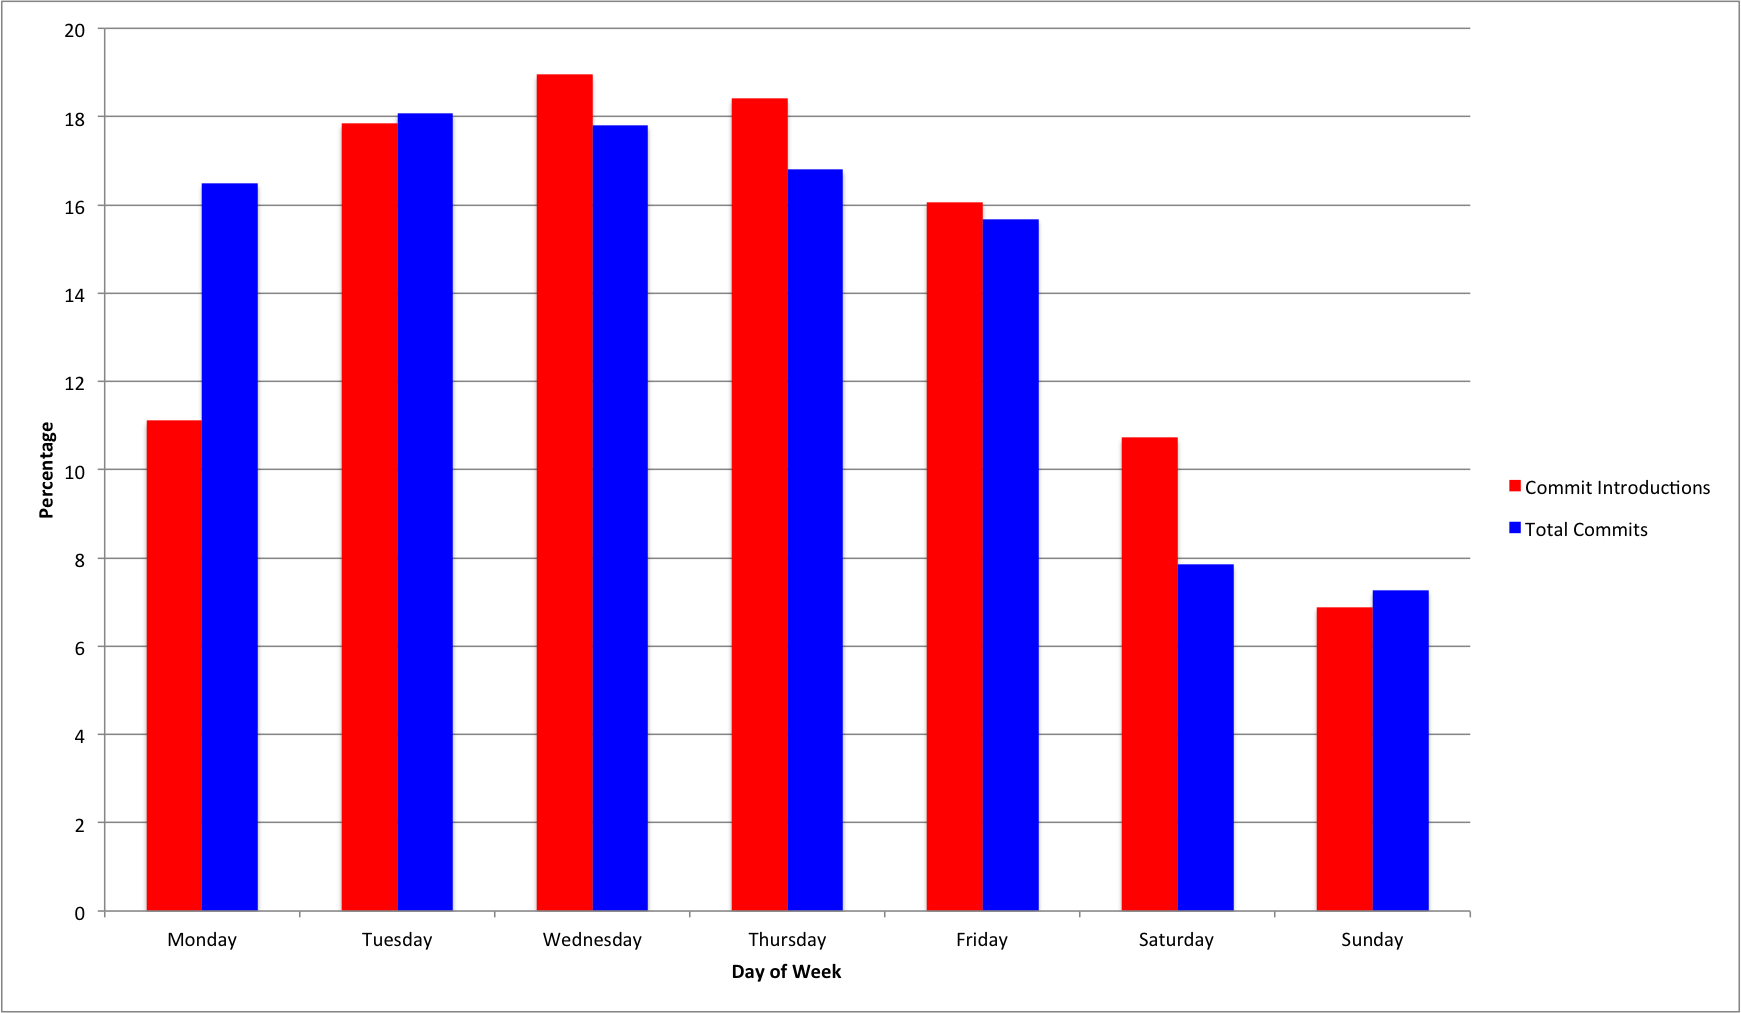
\includegraphics[width=0.45\textwidth]{linux_bug_introduction_day_of_week.png}
\end{center}
\caption{Linux percentage of bug introductions and percentage of total commits per day}
\label{fig-linux-weekday}
\end{figure}

\begin{figure}
\begin{center}
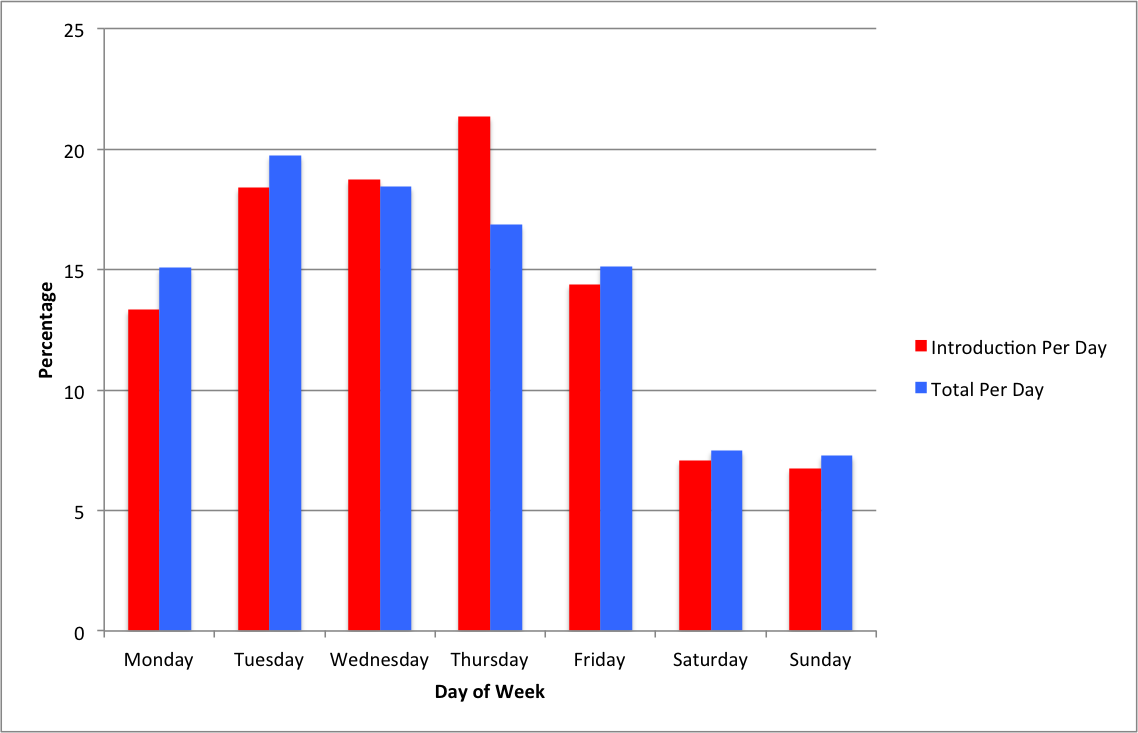
\includegraphics[width=0.45\textwidth]{firefox_bug_introduction_day_of_week.png}
\end{center}
\caption{Firefox percentage of bug introductions and percentage of total commits per day}
\label{fig-firefox-weekday}
\end{figure}

\paragraph{Day-of-week Results} Having determined our false positive rate, 
we continue by presenting the results of our analysis.  First, we
determine if the day of the week has any impact on the likelihood of
producing bugs. For the following graphs, the percentage of
introduction commits indicates the amount of commits which are bug
introductions, as a propostion of the total number of
commits. Figure~\ref{fig-linux-weekday} presents our results for
Linux. We see that Saturday is the worst day, followed by Thursday,
while Monday has the fewest percentage of bug introductions. The
results for Firefox are shown in Figure~\ref{fig-firefox-weekday} and
agree with Thursday being one of the worst days, while Monday is the
best day for committing changes which do not introduce bugs. A
possible explanation is that developers rest over the weekend and have
ample time to think about the problem before coding a solution on
Monday, when they know exactly what to do. Per-day bugginess may also
be correlated with the size of the change, which we plan to investigate
later, as an addition to our technique.

\begin{figure}
\begin{center}
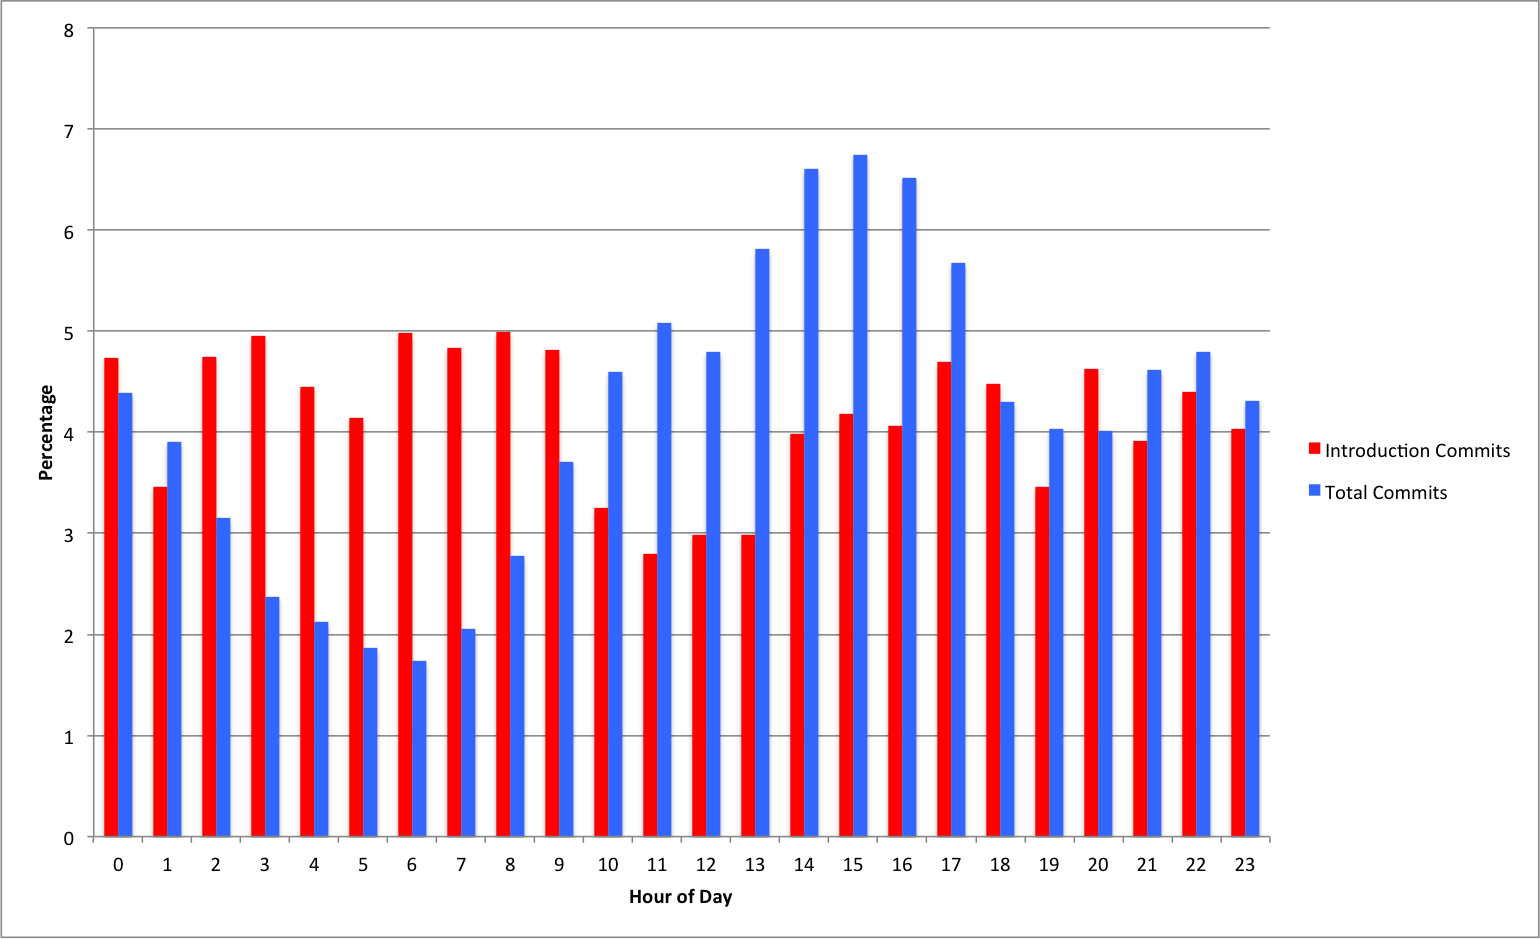
\includegraphics[width=0.45\textwidth]{linux_hour_of_day.png}
\end{center}
\caption{Linux percentage of bug introductions and percentage of total commits per hour}
\label{fig-linux-hour}
\end{figure}

\begin{figure}
\begin{center}
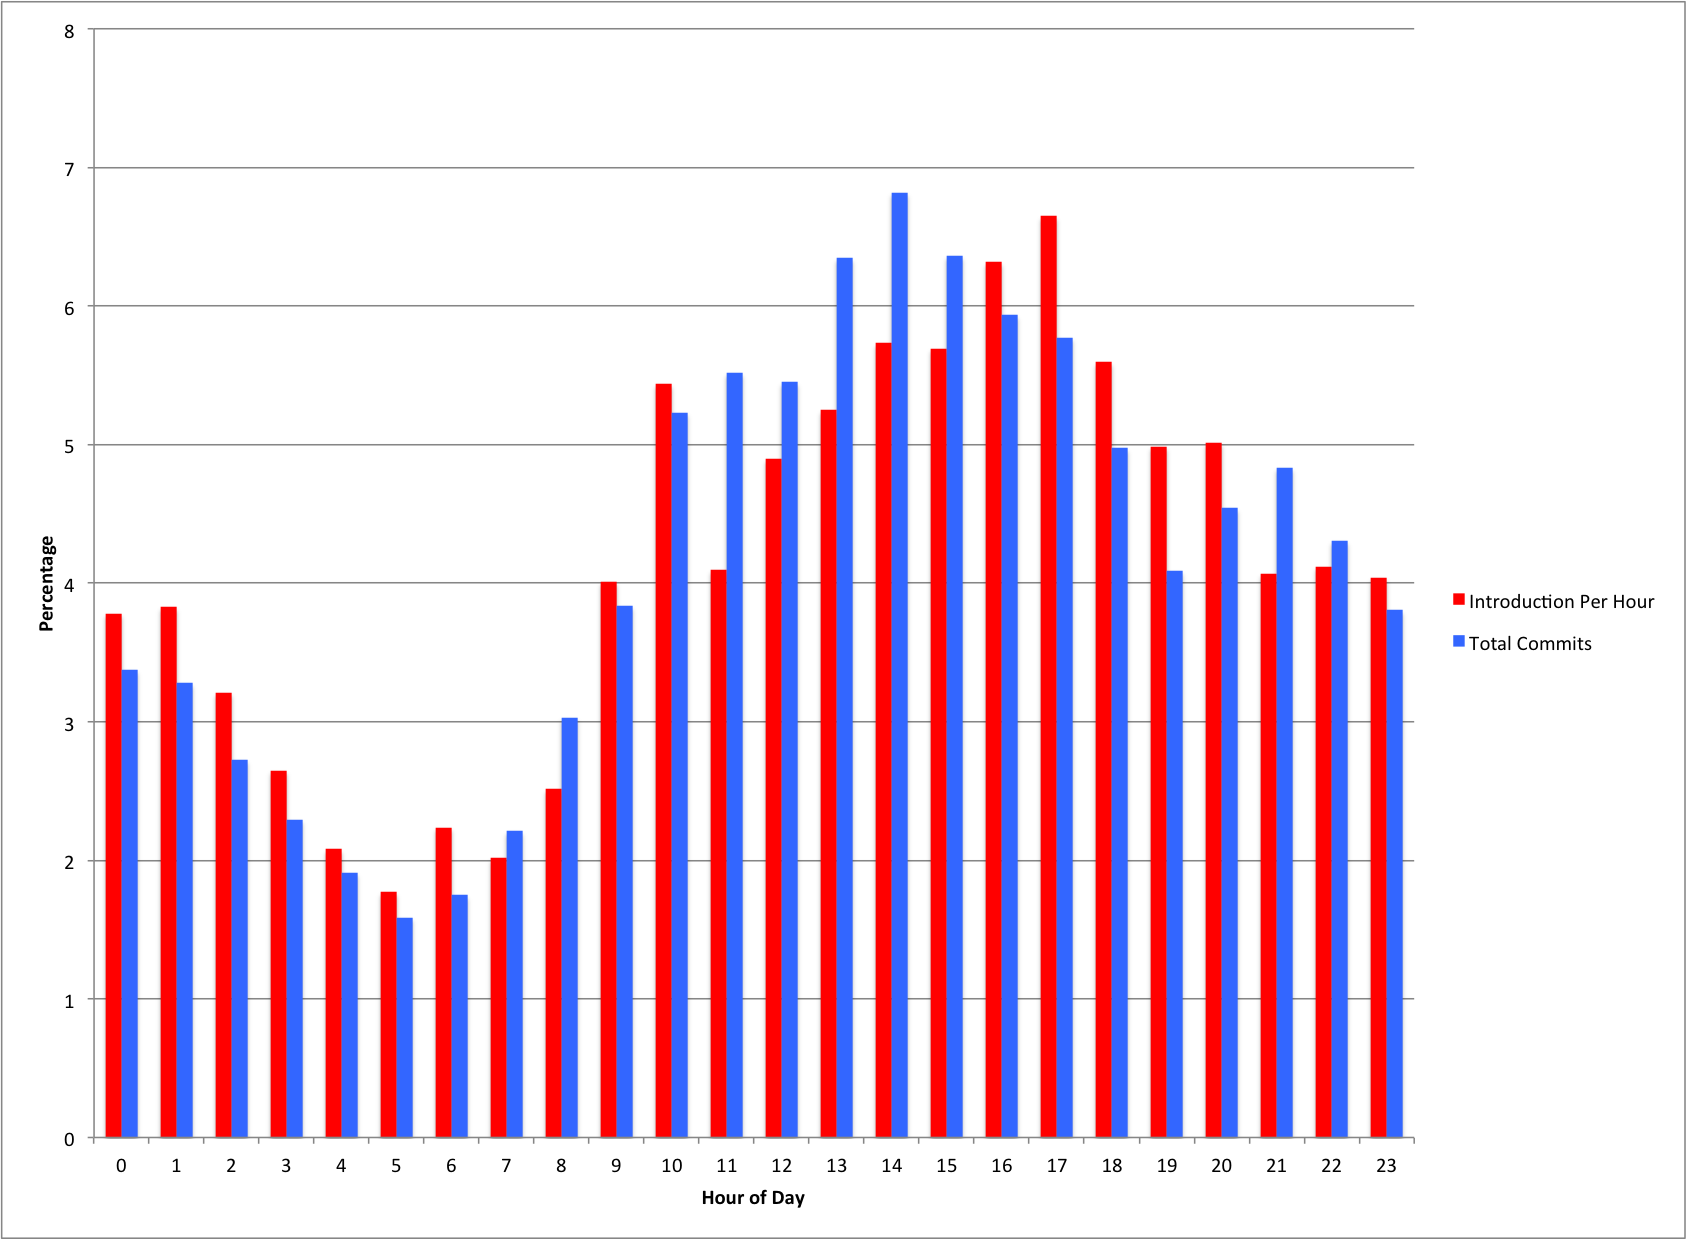
\includegraphics[width=0.45\textwidth]{firefox_hour_of_day.png}
\end{center}
\caption{Firefox percentage of bug introductions and percentage of total commits per hour}
\label{fig-firefox-hour}
\end{figure}

\paragraph{Time-of-day Results} We next investigated whether the hour of a commit has any impact on
its bugginess. Figures~\ref{fig-linux-hour} and~\ref{fig-firefox-hour}
present results from Linux and Firefox, respectively. Both figures
show a significant increase in the amount of commits which introduce a
bug between midnight and 9AM. After 9AM, there is a significant
reduction in the amount of bug introductions between 11AM and 3PM.
However, after 3PM, the likelihood of bug introductions fluctuates
from hour to hour. This result is not very surprising, since tired
programmers are more likely to produce mistakes. It does, however,
indicate the hours that programmers are at the peak of their
productiveness, in terms of not creating additional bugs.

\begin{figure}
\begin{center}
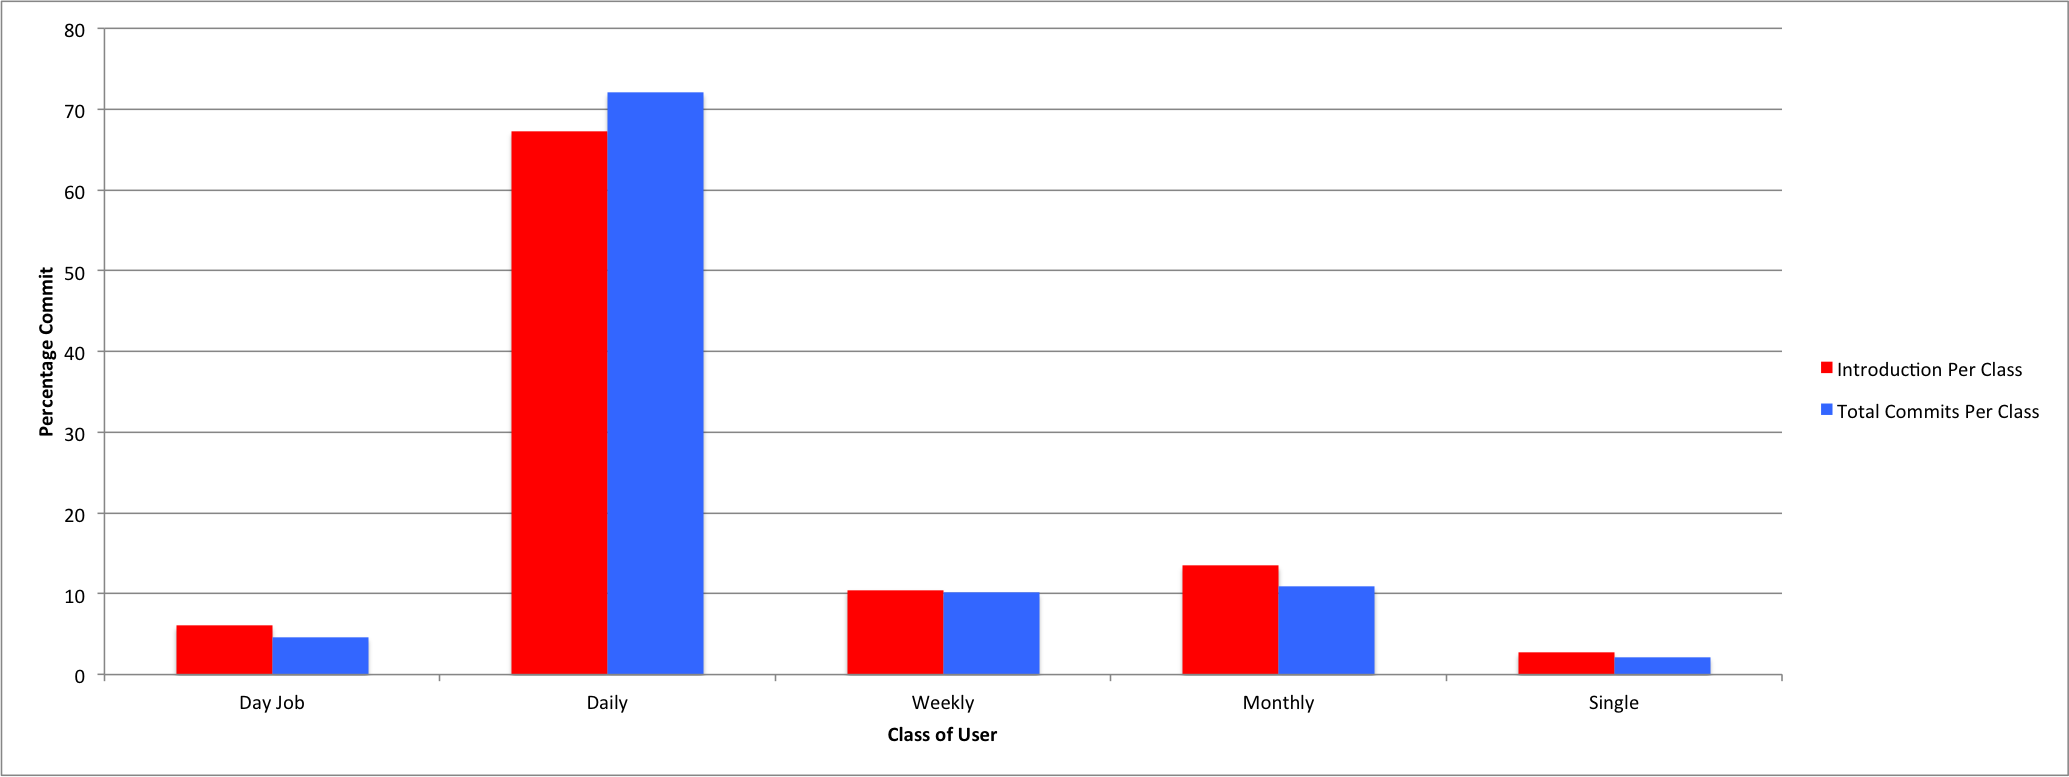
\includegraphics[width=0.45\textwidth]{linux_per_class.png}
\end{center}
\caption{Linux percentage of bug introductions and percentage of total commits per author classification}
\label{fig-linux-class}
\end{figure}

\begin{figure}
\begin{center}
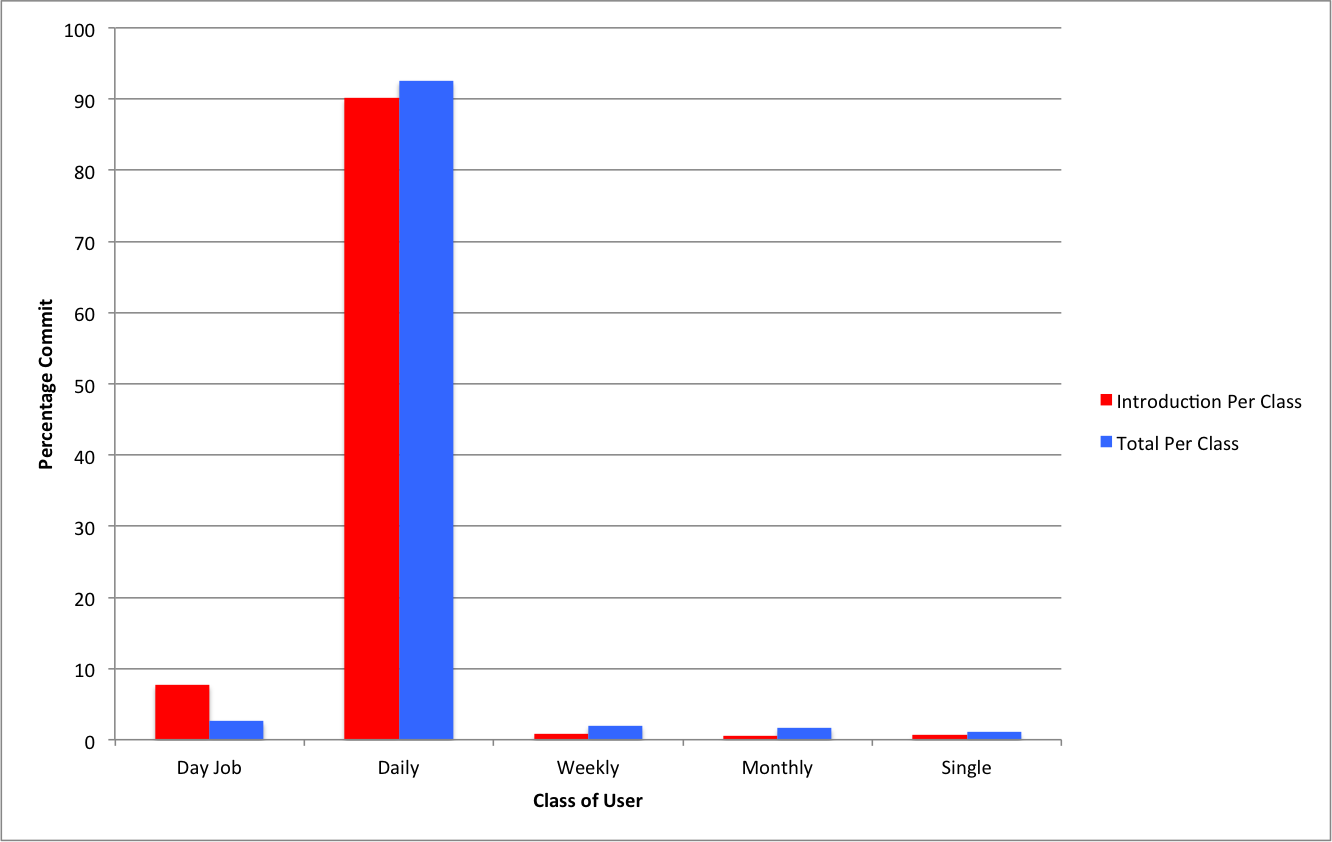
\includegraphics[width=0.45\textwidth]{firefox_per_class.png}
\end{center}
\caption{Firefox percentage of bug introductions and percentage of total commits per author classification}
\label{fig-firefox-class}
\end{figure}

\paragraph{Developer Activity Classification} 
We then investigated how each classification of developers fare in
terms of their likelihood of creating a
bug. Figures~\ref{fig-linux-class} and~\ref{fig-firefox-class} present
our results from Linux and Firefox, respectively.  They show that
developers who commit changes daily, but not as their day job,
contribute significantly to both projects. We believe that this
characteristic should be shared by most open-source projects. Also,
note that for both projects, the daily developers are less likely to
produce bugs, while day-job developers
are more likely to produce bugs. % why do we know this?
A possible cause is that day-job developers are required to make changes,
while the daily developers are motivated purely by interest, and
unlikely to be pressured to fix bugs on any particular schedule.

% we need to say what the two bars mean in the figure.

\begin{figure}
\begin{center}
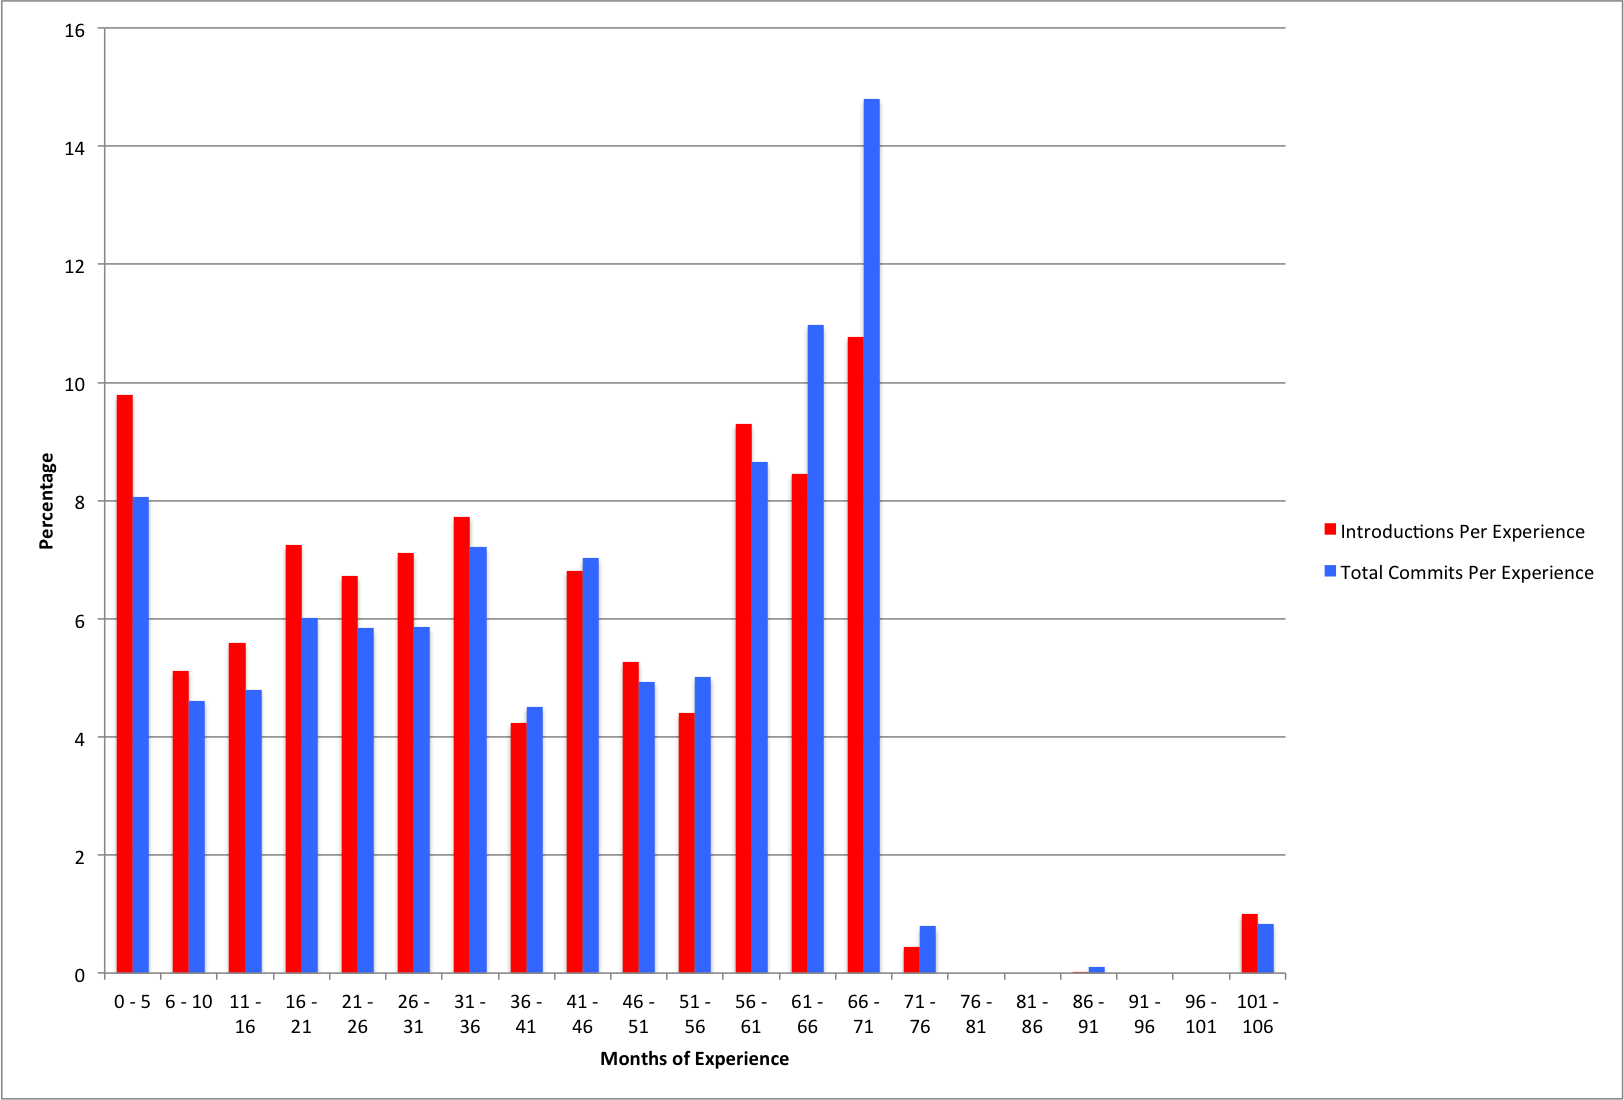
\includegraphics[width=0.45\textwidth]{linux_day_per_experience.png}
\end{center}
\caption{Linux percentage of bug introductions and percentage of total commits per author experience}
\label{fig-linux-experience}
\end{figure}

\begin{figure}
\begin{center}
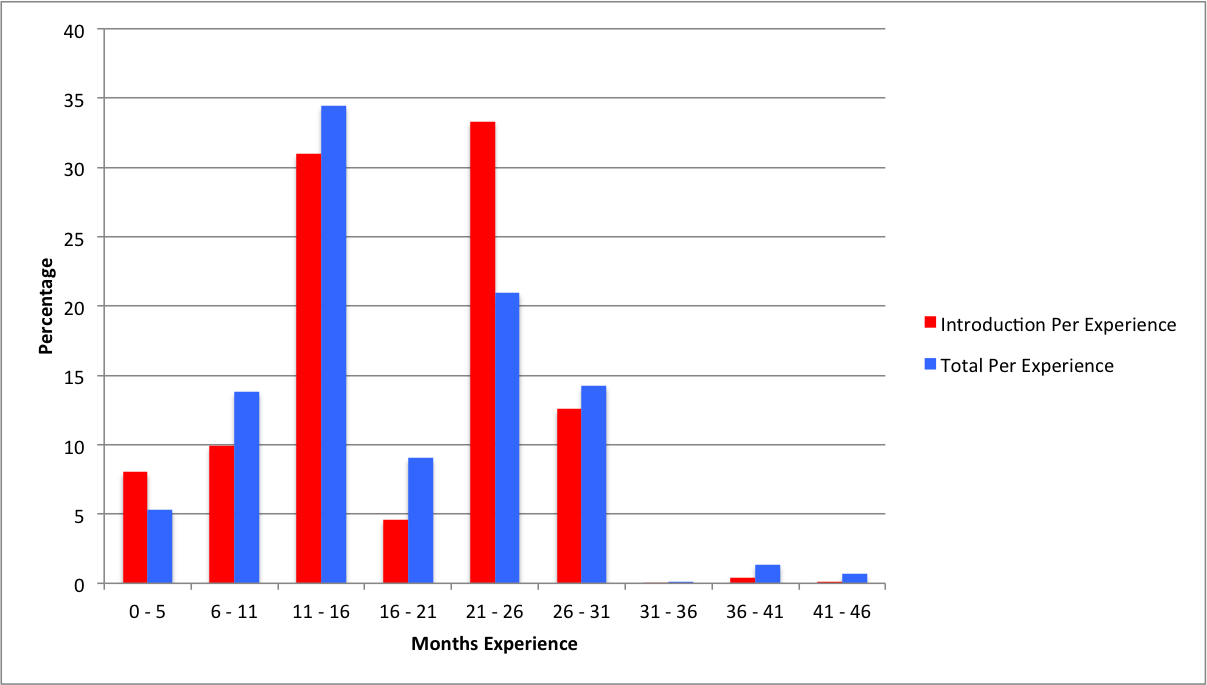
\includegraphics[width=0.45\textwidth]{firefox_day_per_experience.png}
\end{center}
\caption{Firefox percentage of bug introductions and percentage of total commits per author experience}
\label{fig-firefox-experience}
\end{figure}

\paragraph{Developer Experience Classification}
The final head-to-head comparison we performed is based on the amount
of experience per author. We divided them up into 6-month intervals. 
Our results from Linux and Firefox are shown in Figure
\ref{fig-linux-experience} and Figure \ref{fig-firefox-experience}
respectfully. For Linux authors with less than 2 years of experience
are more likely to commit a bug while after 2 years the likelihood
decreases. However the authors which committed throughout the history
of the project are more likely to commit a bug which may be because
they wrote the majority of the code. For Firefox, again the
developers with less than 6 months of experience are more likely to
commit a bug. The is a spike between 21 and 26 months as well. We
believe these results may not be accurate due to the possiblity of
our experience metric being crude and not representative of the 
actual experience with the project.

\begin{figure}
\begin{center}
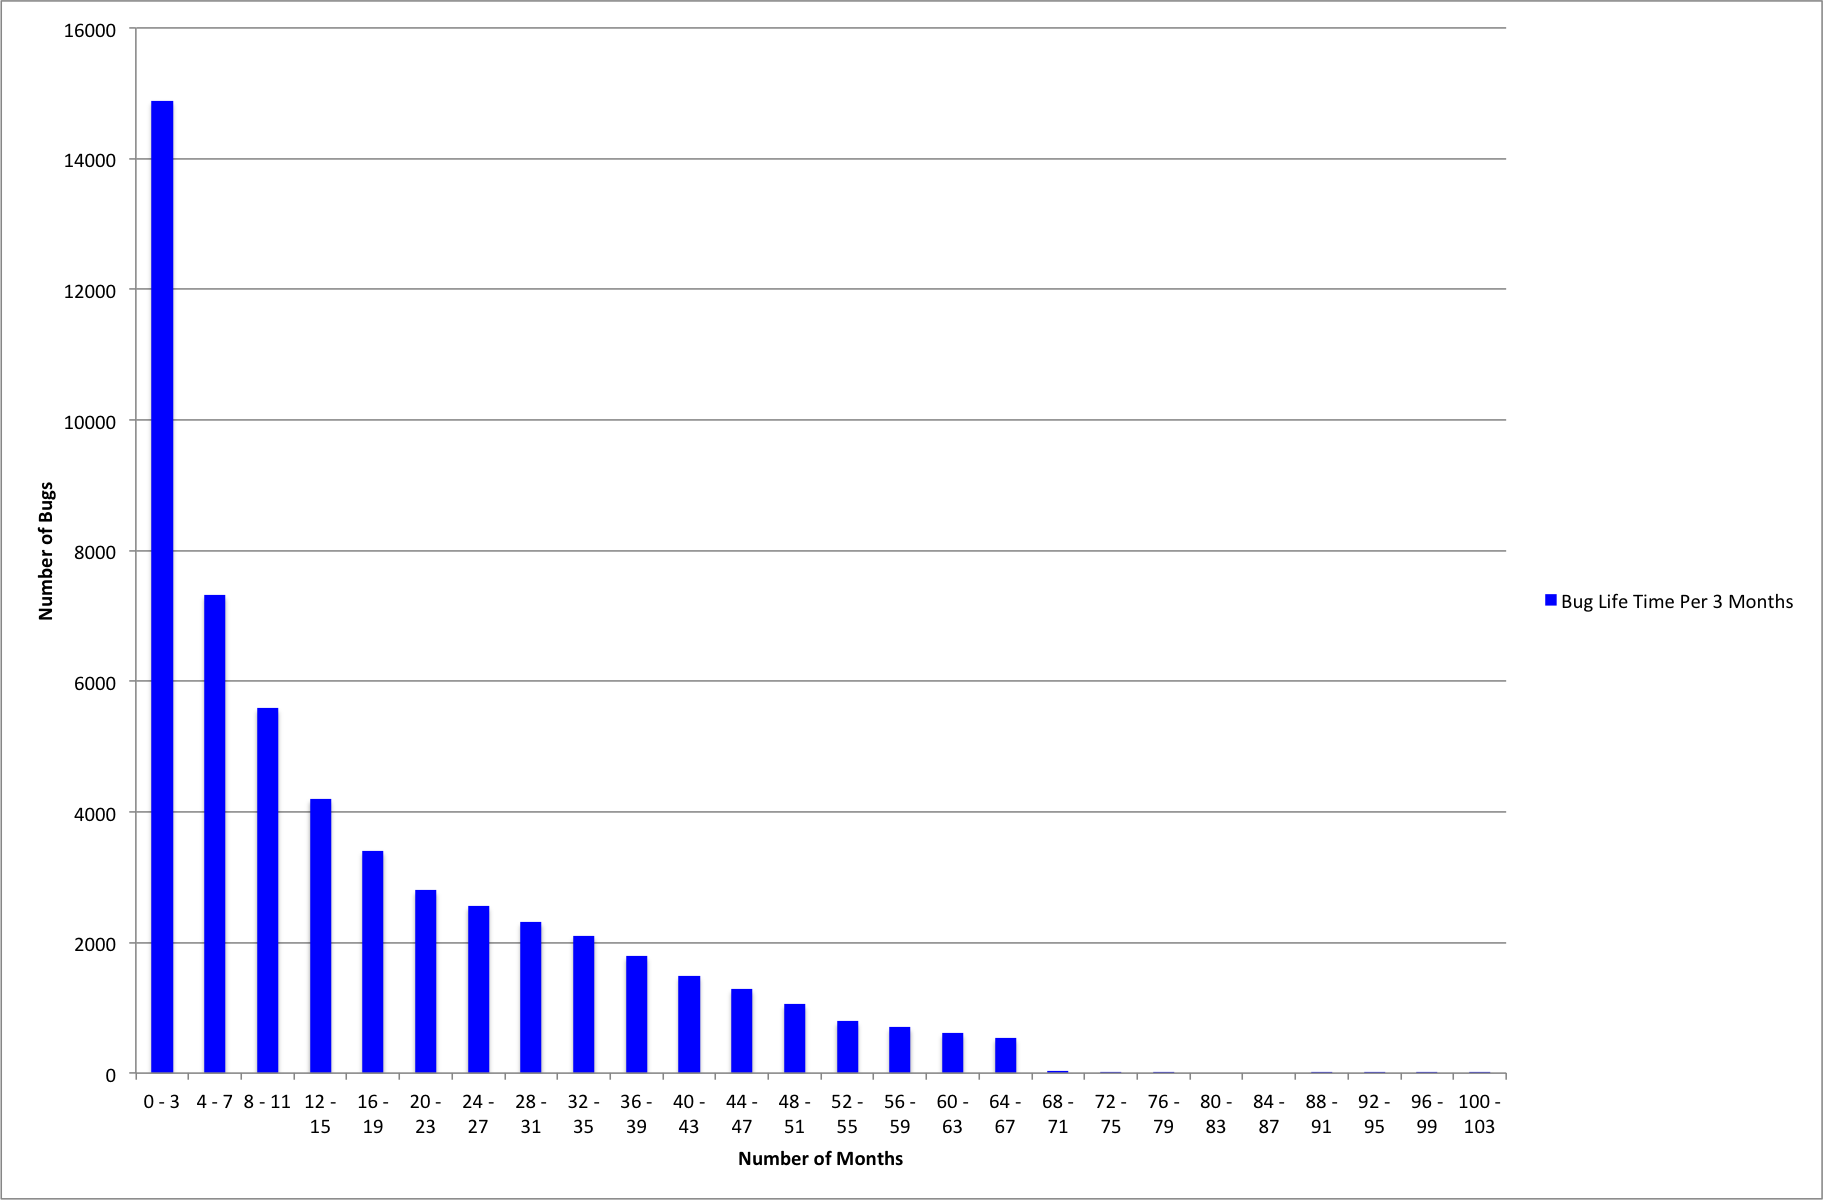
\includegraphics[width=0.45\textwidth]{linux_bug_life.png}
\end{center}
\caption{Linux number of bugs against bug lifetimes in months}
\label{fig-linux-buglife}
\end{figure}

\begin{figure}
\begin{center}
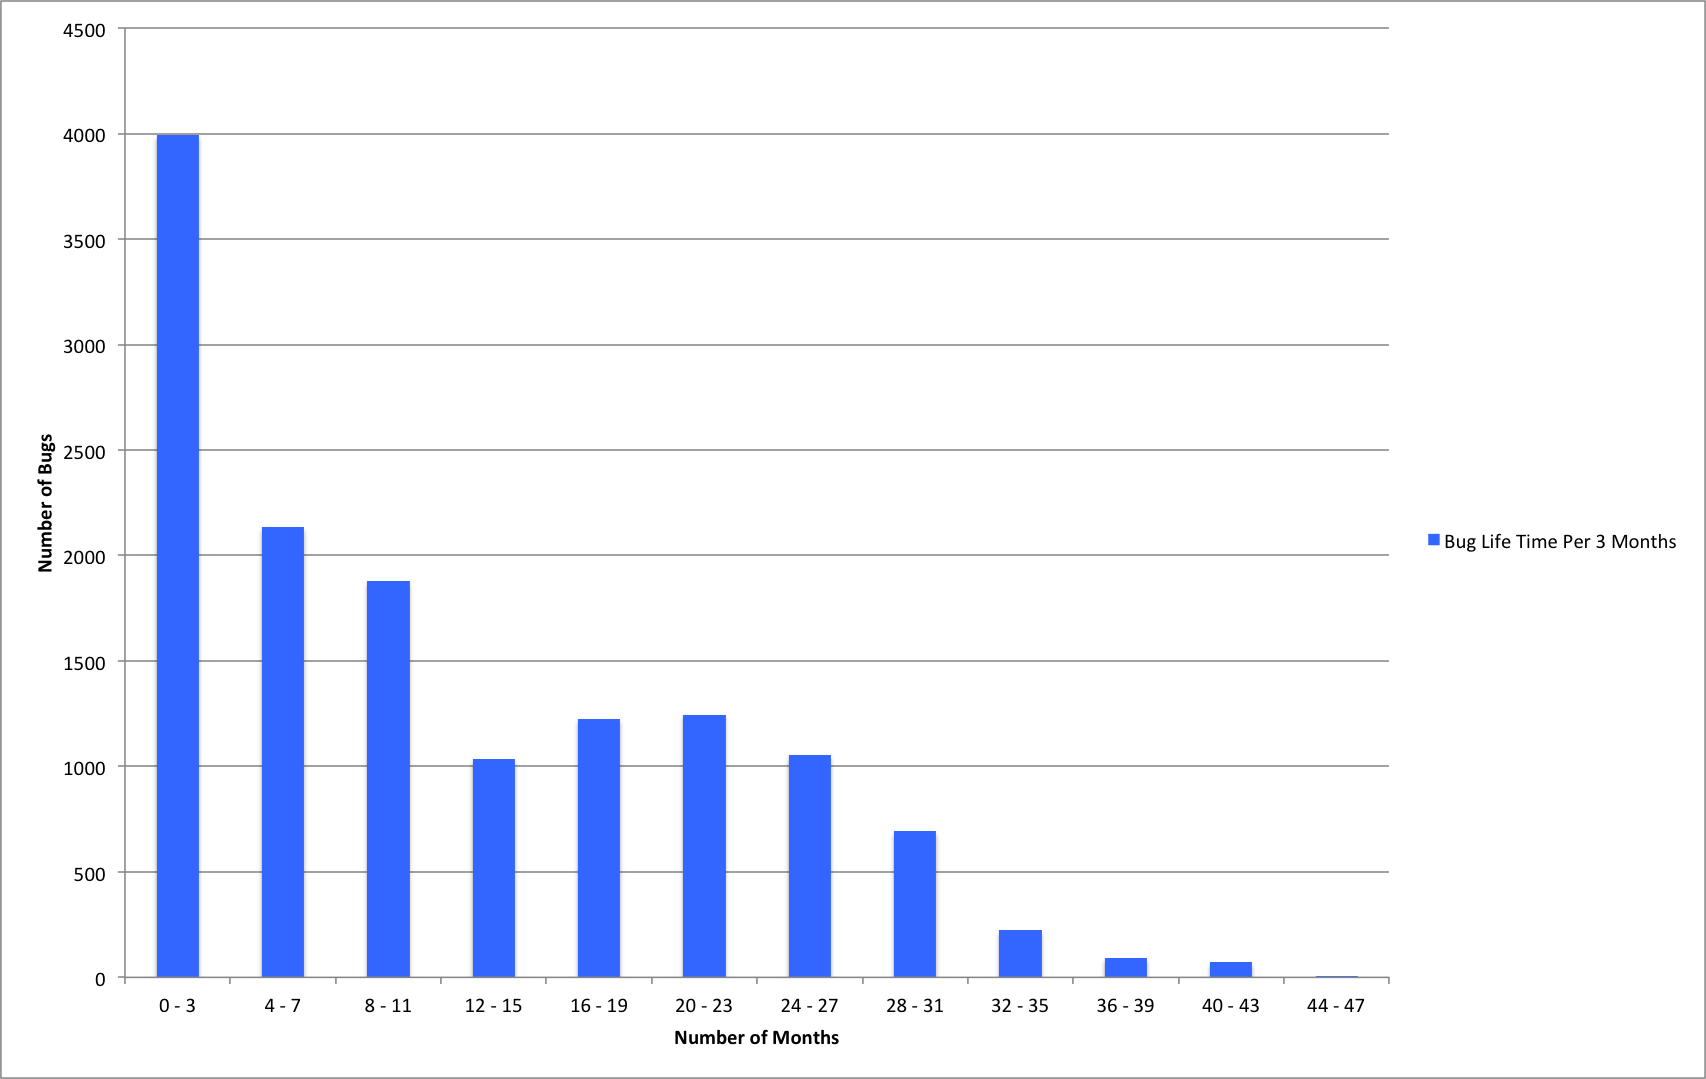
\includegraphics[width=0.45\textwidth]{firefox_bug_life.png}
\end{center}
\caption{Firefox number of bugs against bug lifetimes in months}
\label{fig-firefox-buglife}
\end{figure}

Finally we determined the bug lifetimes for both projects to contrast
them to previous work. We plotted the number of bugs for each lifetime
divided into 4 month intervals. The results for Linux are shown in
Figure \ref{fig-linux-buglife}, the average bug lifetime is 1.39
years. The results for Firefox are shown in Figure
\ref{fig-firefox-buglife}, with an average bug lifetime of 0.97
years. This shows a reduction in the average bug lifetime for Linux (in
2002 the average lifetime was 1.8 years). This indicates that
developers are improving as their development process becomes more
refined. We also see the average lifetime is lower for Firefox, this
may be due to the complexity of the software, size of the software or
the amount of users (the more users and complex, the more likely bugs will be
revealed).
